% Generated from tex/chapters/ch04/08_構築技術.tex for the SWEBOK structure tree
\subsubsection{状態に基づく構築技法と表駆動構築技法}

状態に基づくプログラミングは、有限状態機械を使ってプログラムの振る舞いを表す技法である。状態、イベント、遷移、動作を明確にすることで、複雑な分岐を整理できる。状態遷移図は、仕様、実装、デバッグ、文書化で使える。

表駆動方式は、複雑な \texttt{if} 文や \texttt{case} 文の代わりに、表を使って情報を表す方法である。条件と処理の対応を表にまとめると、ロジックが見通しやすく、変更もしやすくなることがある。表駆動では、何を表に入れるか、どのように効率よく表を参照するかが重要である。

\begin{figure}[htbp]
\centering
\IfFileExists{assets/generated_figures/ch04/fig-ch04-11.png}{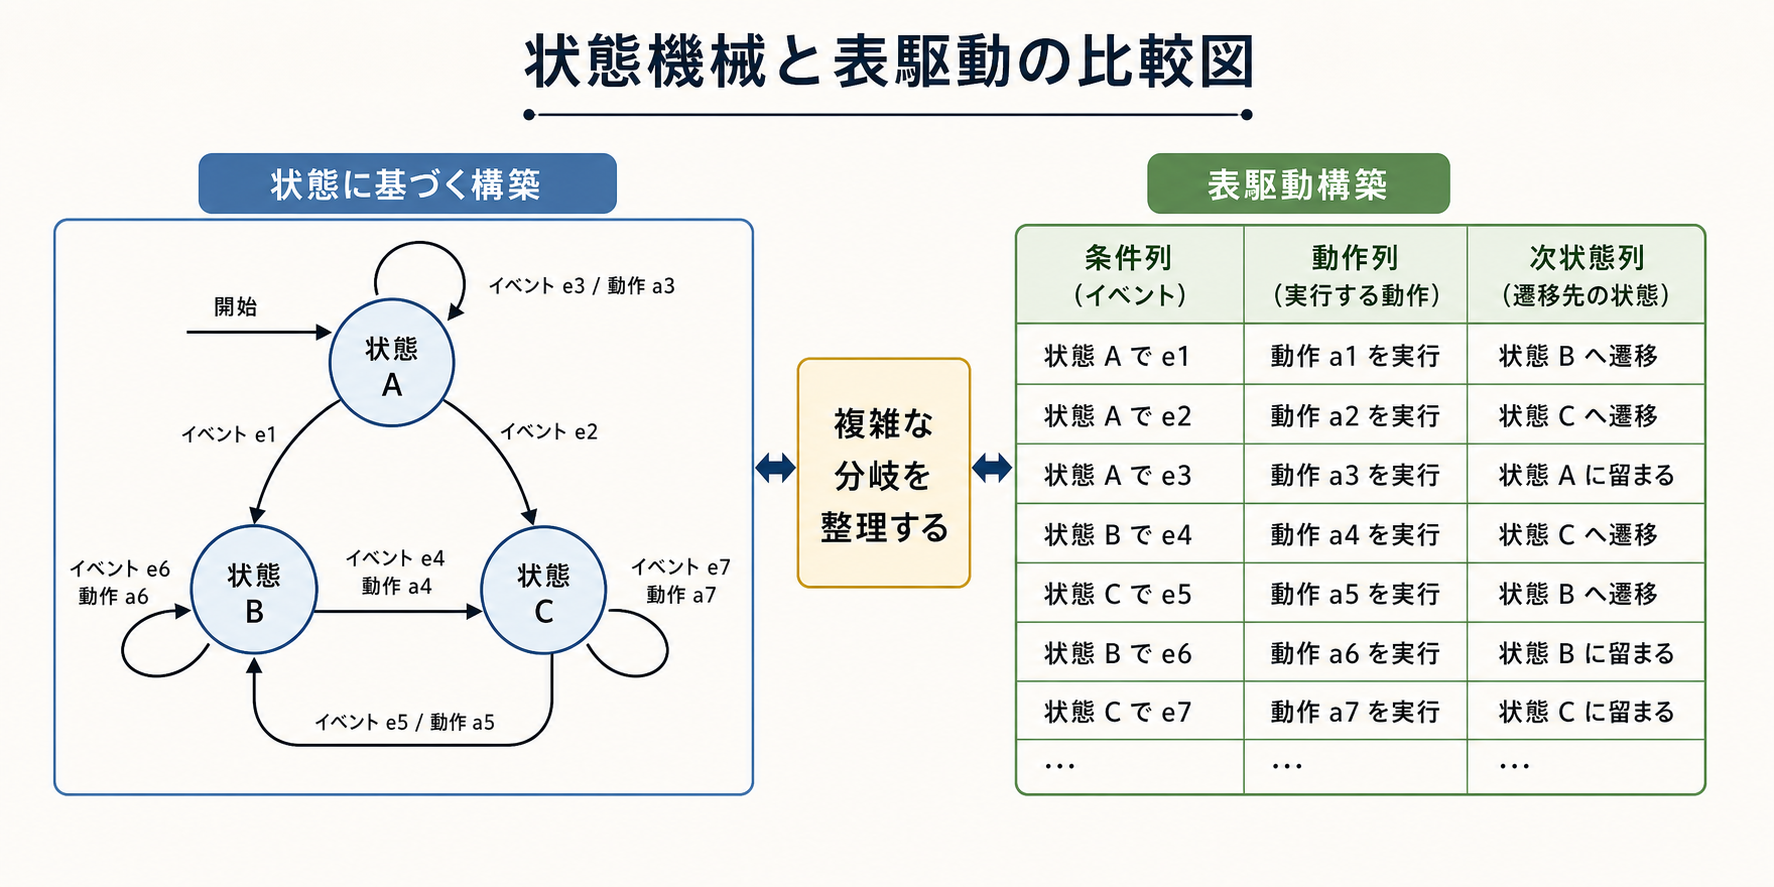
\includegraphics[width=0.96\linewidth]{assets/generated_figures/ch04/fig-ch04-11.png}}{\fbox{\parbox[c][48mm][c]{0.9\linewidth}{\centering 画像生成待ち\\状態機械と表駆動の比較図}}}
\caption{状態機械と表駆動の比較図}
\label{fig:ch04-11}
\end{figure}
